\subsection{\textbf{Latar Belakang}}

Terumbu karang adalah ekosistem bawah laut yang terbentuk dari sekumpulan karang. Selain berfungsi sebagai ekosistem di bawah laut, terumbu karang juga berfungsi sebagai pemecah gelombang. Sebagian besar kepulauan di wilayah pasifik di kelilingi oleh terumbu karang yang tumbuh di laut dangkal yang dekat dengan pantai \cite{DemirbilekBoussinesq}.

Gelombang yang melewati terumbu karang akan teredam kecepatannya \cite{DemirbilekReport}. Hal ini akan mempengaruhi naiknya gelombang ke daratan di atas batas normal gelombang \emph{runup}\cite{nielsen1991wave}. Teredamnya kecepatan gelombang disebabkan oleh bertumbukannya dasar gelombang dengan karang. Dalam beberapa kasus, hal ini menyebabkan pecahnya gelombang \cite{DemirbilekReport}. Pada gambar.\ref{fig:hawai_coral} dapat dilihat pecahnya gelombang yang terjadi di atas karang.

\begin{figure}[htp]
    \begin{center}
        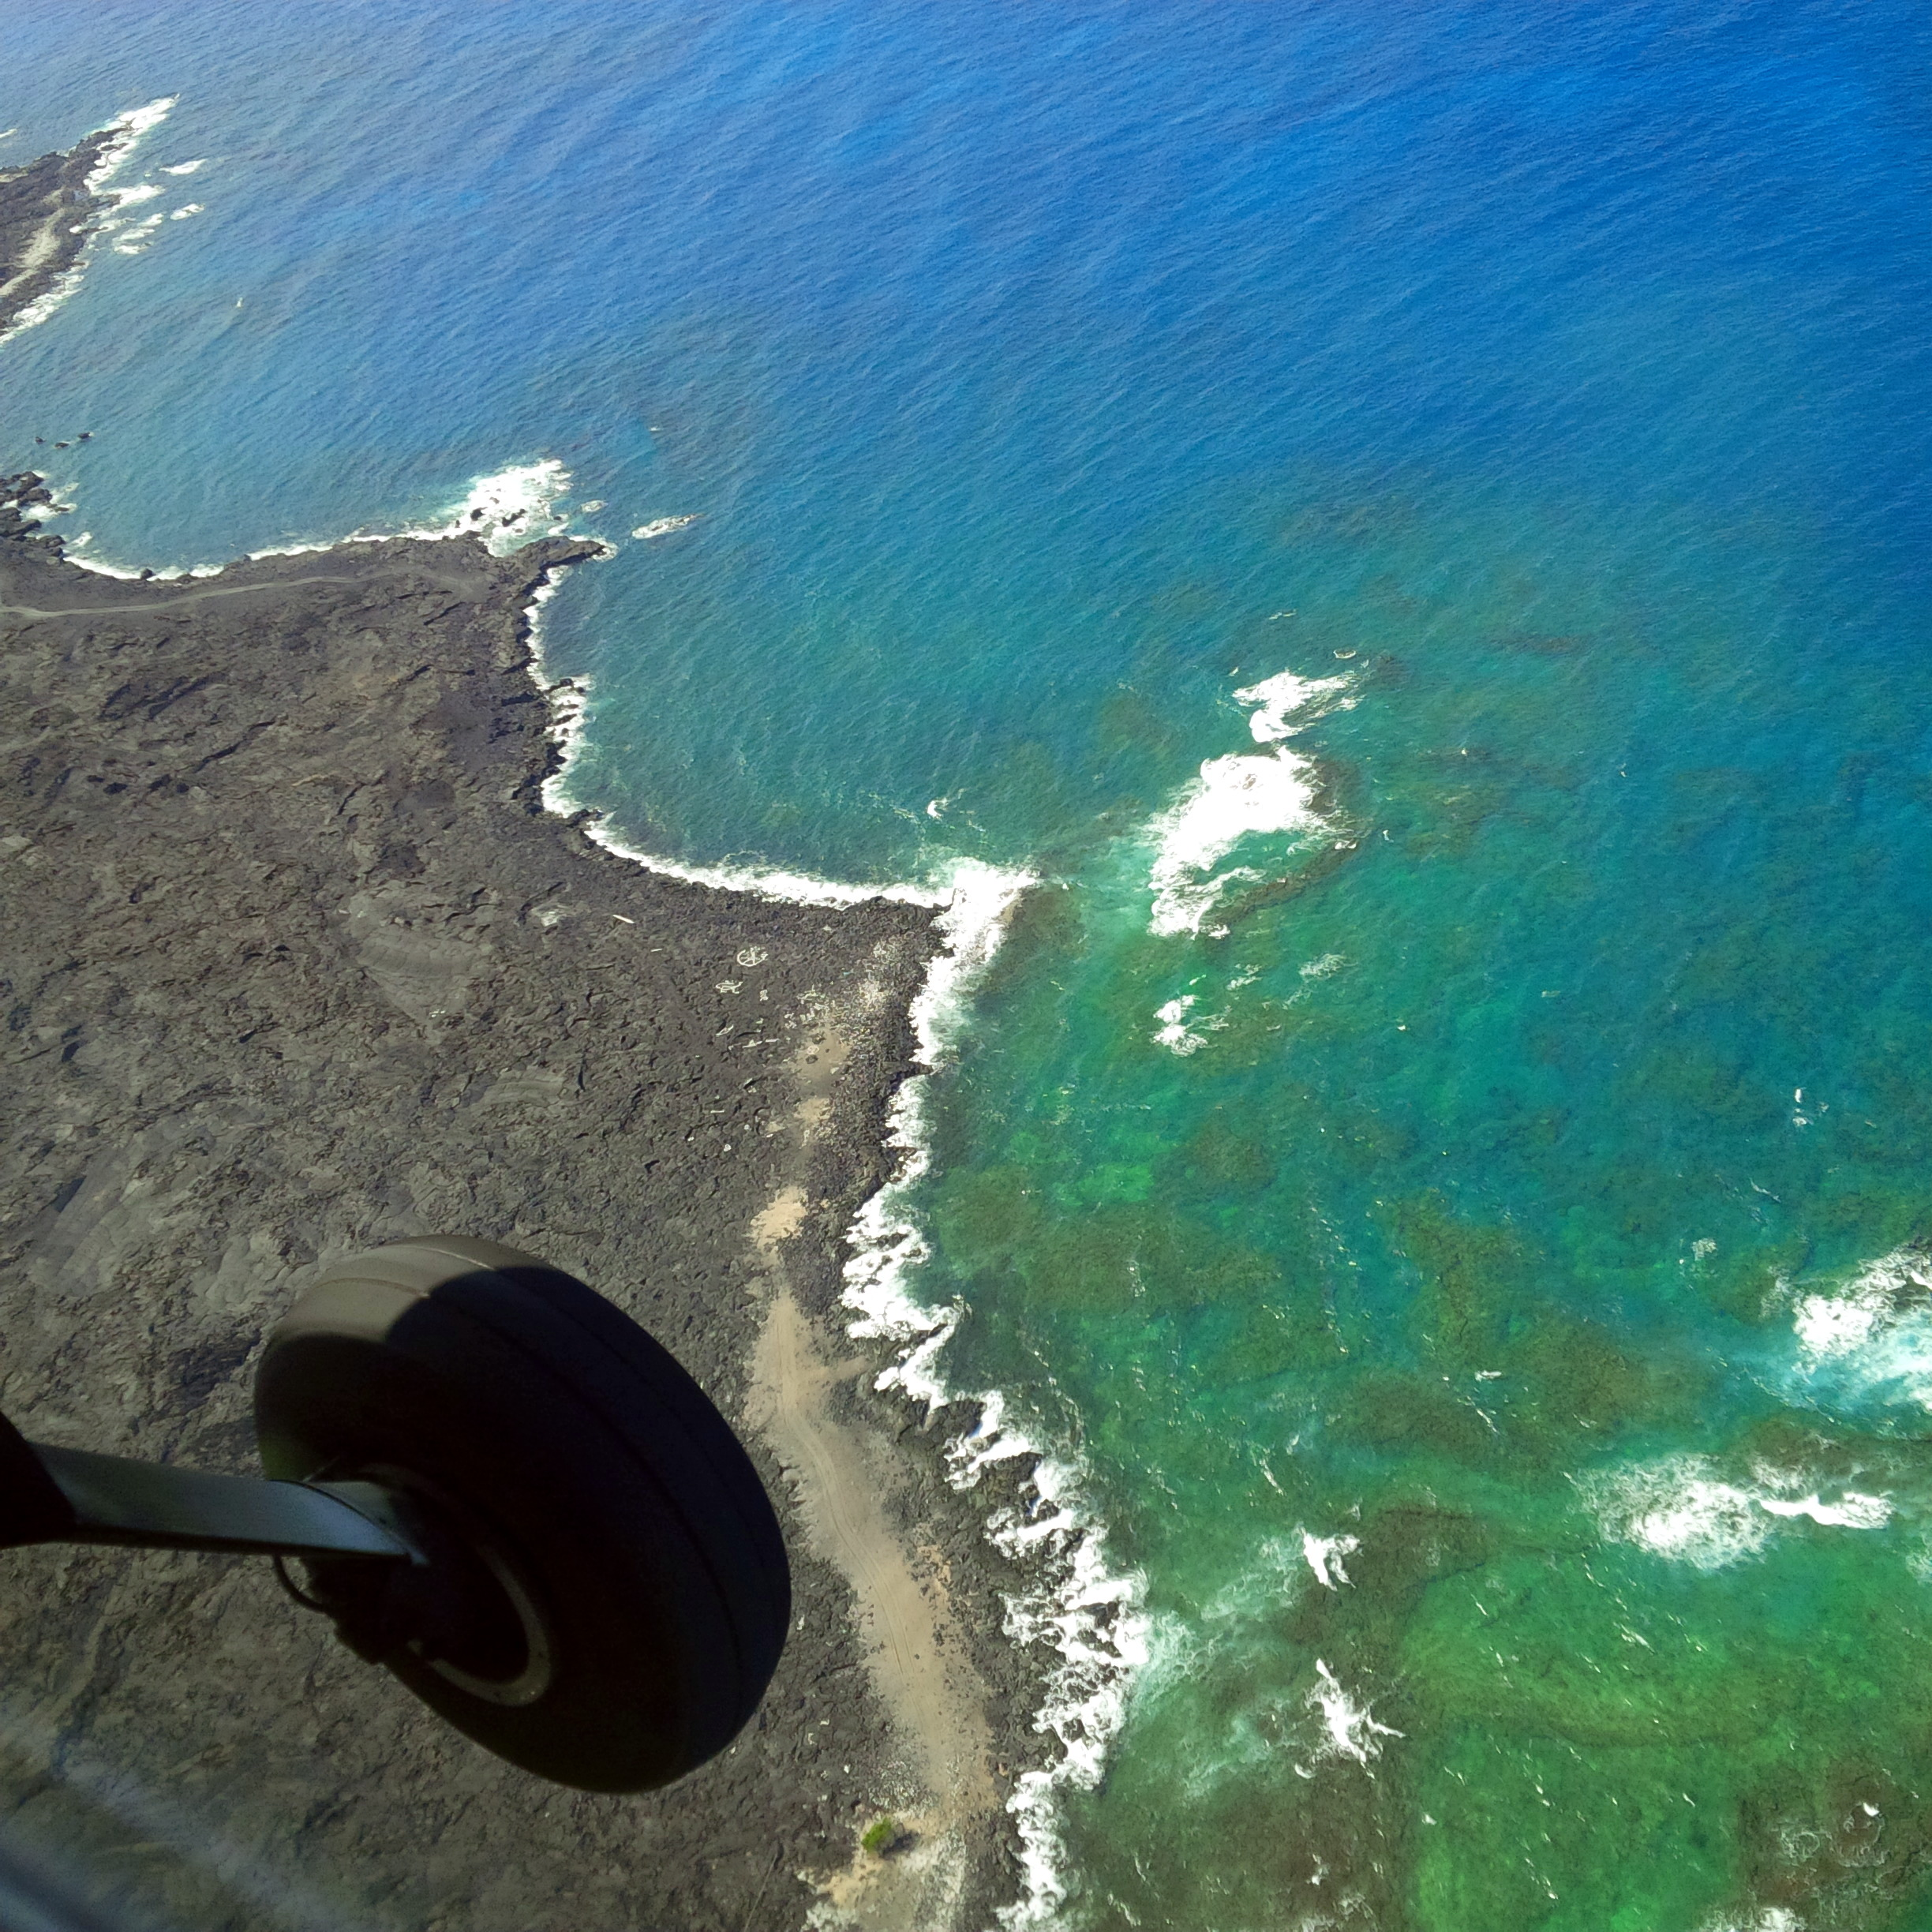
\includegraphics[scale=0.1]{./images/hawai_coral.jpg}
    \end{center}
    \caption{Terumbu Karang di tepi pantai di sekitar Hawai.}
    \label{fig:hawai_coral}
\end{figure}
\FloatBarrier
Efektifitas dari terumbu karang dalam meredam gelombang masih menjadi perdebatan para peneliti. penelitian ini sudah pernah dilakukan oleh Yau et al pada tahun 2012 dengan menggunakan model \emph{Boussinesq} 1 dimensi untuk memodelkan transformasi gelombang saat melewati terumbu karang. Namun cara mempelajari ini tergolong mahal dan membutuhkan pemodelan matematika yang kompleks untuk memodelkan pecahnya gelombang\cite{YAO201230}

Dalam memprediksi tinggi gelombang \emph{runup} pada terumbu karang digunakan dua metode yang masih tergolong baru yaitu metode pendekatan klasik yang dilakukan secara analitis yakni dengan melakukan eksperimen dan observasi kemudian, menentukan model matematika yang tepat. Model yang demikian sulit untuk dikembangkan karena beradaptasi dengan kondisi lingkungan yang berbeda. Prediksi yang didapat dari model yang demikian pun masih belum sempurna \cite{DemirbilekBoussinesq} Sedangkan metode yang kedua adalah dengan  pendekatan \emph{soft computing}.\\

{\textbf{Topik dan Batasan}}

Pada penelitian ini `menggunakan metode pembelajaran mesin yaitu dengan metode \emph{Feed forward neural network}(\emph{supervised learning}) untuk memprediksi tinggi \emph{runup} gelombang. data yang digunakan adalah data analisa observasi gelombang yang diambil dari laboratorium dinamika oleh Demirbilek pada tahun 2007\cite{DemirbilekReport}.\\

{\textbf{Tujuan}}

Tujuan dari tugas akhir ini adalah bagaimana Membuat model prediksi dengan menggunakan metode \emph{Feed forward Neural Network} dengan menggunakan data hasil eksperimen pada laboratorium  dinamika kemudian mengevaluasi hasil prediksi dengan mengevaluasi model dengan mencari  akurasi dari model prediksi yang telah dibuat.

